\documentclass{./../div_teaching_slides}

\begin{document}
\title{ECON 340 \\ Economic Research Methods}
\author{Div Bhagia}
\date{Lecture 14: Hypothesis Testing \& p-Values}

%%%%%%%%%%%% 
\begin{frame}[noframenumbering, plain]
\maketitle
\end{frame}


%%%%%%%%%%%%
\begin{frame}{Sample Mean Distribution}
Let $X_1, X_2,..., X_n$ denote independent random draws (random sample) from a population with mean $\mu$ and variance $\sigma^2$. 
$$ \bar{X} \sim N(\mu, \sigma^2/n)  $$
The sample mean  $\bar{X}$ is normally distributed when the underlying population is normal \textit{or} sample size is large, say $n \geq 100$ (CLT).
\end{frame}

%%%%%%%%%%%%
\begin{frame}{Blood Pressure in Massachusetts}
\centering
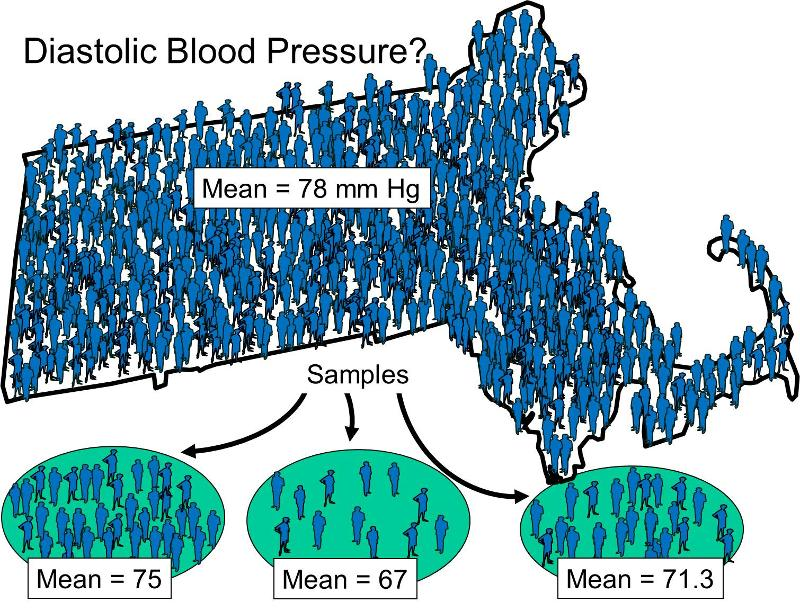
\includegraphics[scale=0.35]{Sampling3.jpg}
\end{frame}

%%%%%%%%%%%%
\begin{frame}{Blood Pressure in Massachusetts}
Let's say we picked a random sample of 100 people from Massachusetts and took their blood pressure. \\~\\
We found that the average diastolic blood pressure in our sample was 75 i.e. $\bar{x} = 75$ \\~\\
Let's say our prior was $\mu=78$, but we found $\bar{x}=75$. Can we conclude our prior was wrong? \\~\\
\pause	Not yet! It could be that the true mean was 78, but just by chance we got 75.  We can formally test our ``hypothesis.''
\end{frame}


%%%%%%%%%%%%
\begin{frame}{Hypothesis Testing}
\vspace{-0.5em}
\begin{witemize}
  \item Note that $n=100$. For now, assume we know $\sigma^2 = 552.25$. 
  \item So if our initial hypothesis ($\mu=78$) is correct, then $$\bar{X} \sim N(78, 5.52)$$
  \item To test our hypothesis, say at 10\% level of significance: \\ \vspace{0.1em}
  \begin{witemize}
  \normalsize
  \item Find the 10\% most surprising outcomes, assuming our initial hypothesis is true
  \item If the obtained sample mean $\bar{x}=75$ is in the 10\% most surprising outcomes, agree that we were wrong 
\end{witemize}
\end{witemize}
\end{frame}

%%%%%%%%%%%%
\begin{frame}{Hypothesis Testing}
\begin{witemize}
  \item If 75 is not in the 10\% most surprising outcome.
  \item Then it is quite likely that with a true population mean of 78, we actually got a sample mean of 75.
  \item So we cannot conclude that our initial hypothesis was wrong at least under this criterion.
  \item To make this easy on ourselves, we will find the most surprising outcomes in terms of the standard normal distribution
\end{witemize}
\end{frame}

\begin{frame}{Hypothesis Testing: Recipe}
\begin{enumerate}
\item[1.] We will call our initial hypothesis as the \textbf{null hypothesis}. 
$$ H_0: \mu = 78 $$ \\~\\
We will test this against an \textbf{alternative hypothesis}. Natural alternative here is
$$ H_1: \mu \neq 78 \quad $$ 
\end{enumerate}
\end{frame}

%%%%%%%%%%%%
\begin{frame}{Hypothesis Testing: Recipe}
\begin{enumerate}
\item[2.] Given that our null is true, in this example we know that 
$$ \bar{X} \sim N(78, 5.52)$$ \\~\\
Test statistic under the null: 
$$Z =  \frac{\bar{X} - \mu_0}{\sigma_{\bar{x}}} \sim N(0,1) $$
\end{enumerate}
\end{frame}

\begin{frame}{Hypothesis Testing: Recipe}
\begin{enumerate}
\item[3.] \textbf{Significance level} $\alpha$: determines how surprised do you have to be before you reject the null hypothesis. \\~\\
So our \textbf{rejection region} is $\alpha \%$ of outcomes that are most surprising given the null. \\~\\
\end{enumerate}
\end{frame}

%%%%%%%%%%%%%%%%%%%%
%\begin{frame}{}
%\centering \includegraphics[scale=0.6]{one}
%\end{frame}

%%%%%%%%%%%%%%%%%%%%
\begin{frame}{Rejection Region}
At 10\% level of significance: \\ \vspace{0.5cm}

\begin{tikzpicture}[scale=1]
\begin{axis}[
  no markers, domain=-3:3, samples=100,
  axis lines*=left, xlabel=$Z$, ylabel=$f(Z)$,
  %every axis y label/.style={at=(current axis.above origin),anchor=south},
  height=6cm, width=12cm,
  xtick={-1.64, 0, 1.64}, xticklabels={-1.64, 0, 1.64}, %ytick=\empty,
  enlargelimits=false, clip=false, axis on top,
  ]
  \addplot [very thick,black] {gauss(0, 1)}; 
    \addplot [fill=purple!20, draw=none, domain=-3:-1.64] {gauss(0, 1)} \closedcycle;
    \addplot [fill=purple!20, draw=none, domain=1.64:3] {gauss(0, 1)} \closedcycle;
%\draw[->, line width=1pt](axis cs: 185, 0.0125)--(axis cs: 205, 0.0125);
\node at (axis cs: 1.875, 0.03) { \small 5\%};
\node at (axis cs: -1.875, 0.03) { \small 5\%};
\node at (axis cs: -2,0.24) { \small Rejection};
\node at (axis cs: -2,0.2) { \small Region};
\node at (axis cs: 2,0.24) { \small Rejection};
\node at (axis cs: 2,0.2) { \small Region};
\end{axis}
\draw[<-, solid, thick] (2.1,0.6) -- (1.8,1.8);
\draw[<-, solid, thick] (8.3,0.6) -- (8.6,1.8);
\end{tikzpicture}
\end{frame}



%%%%%%%%%%%%
\begin{frame}{Hypothesis Testing: Recipe}
Here $z_{0.05} = 1.64$ is the \textbf{critical value}. \\~\\
So if our test statistic 
$$ |z| = \left|\frac{\bar{x} - 78}{\sigma_{\bar{x}}}\right| > 1.64 \rightarrow \text{Reject the null} $$
Otherwise, do not reject the null. \\~\\
In our example, we cannot reject the null at 10\% level of significance as $|z|=\left|\frac{75-78}{\sqrt{5.52}}\right| = 1.28<1.64$. 
\end{frame}

%%%%%%%%%%%%
\begin{frame}{p-Value}
\vspace{-0.25cm}
p-value is defined as the probability of randomly drawing an outcome as surprising or more surprising given the null. \\ \vspace{0.75cm}
\begin{tikzpicture}[scale=1]
\begin{axis}[
  no markers, domain=-3:3, samples=100,
  axis lines*=left, xlabel=$Z$, ylabel=$f(Z)$,
  %every axis y label/.style={at=(current axis.above origin),anchor=south},
  height=6cm, width=12cm,
  xtick={-1.28, 0, 1.28}, xticklabels={-1.28, 0, 1.28}, %ytick=\empty,
  enlargelimits=false, clip=false, axis on top,
  ]
  \addplot [very thick,black] {gauss(0, 1)}; 
    \addplot [fill=purple!20, draw=none, domain=-3:-1.28] {gauss(0, 1)} \closedcycle;
    \addplot [fill=purple!20, draw=none, domain=1.28:3] {gauss(0, 1)} \closedcycle;
%\draw[->, line width=1pt](axis cs: 185, 0.0125)--(axis cs: 205, 0.0125);
\node at (axis cs: 1.75, 0.04) { \small 10\%};
\node at (axis cs: -1.75, 0.04) { \small 10\%};
\node at (axis cs: -1.875,0.24) { \small More};
\node at (axis cs: -1.875,0.2) { \small Surprising};
\node at (axis cs: 1.875,0.24) { \small More};
\node at (axis cs: 1.875,0.2) { \small Surprising};
\end{axis}
\draw[<-, solid, thick] (2.5,0.8) -- (2.1,1.8);
\draw[<-, solid, thick] (8,0.8) -- (8.3,1.8);
\end{tikzpicture}

\end{frame}

%%%%%%%%%%%%
\begin{frame}{p-Value: Recipe}

\begin{align*}
 \text{p-value} &= 2 P\left(Z > \left|\frac{\bar{x} - 78}{\sigma_{\bar{x}}}\right| | H_0: \mu = 78 \right) \\
 &= 2P(Z>1.28) = 0.2
\end{align*}
\vspace{1em}

If $p$-value $ <\alpha$, we can reject the null at $\alpha$ level of significance.
\end{frame}


%%%%%%%%%%%%
\begin{frame}{What if we don't know $\sigma^2$}
\begin{witemize}
  \item Proceed as before and create a test statistic using $S$:
 $$ T = \frac{\bar{X}-\mu_0}{S/\sqrt{n}} \sim t_{n-1} $$ 
\item Reject the null if $|t|> t_{n-1, \alpha/2}$
\item For large n, say $n \geq 100$, standard normal distribution approximates the $t$-distribution well
\item So with large samples, we calculate a $t$-statistic but can just look at the standard normal table for critical values
\end{witemize}
\end{frame}

%%%%%%%%%%%%
\begin{frame}{Next up}
\vspace{-0.5em}
\begin{witemize}
  \item Next class: Review for the midterm
  \item Midterm exam on Thurs. Study guide and sample exam uploaded on the course website.
 %\item Research project meetings next to next week on Tues (10/17). Online or in-person, 15-20 minutes slots for each group. I will send details on how to sign up on Canvas. 
\end{witemize}
\end{frame}

\end{document}